\documentclass{beamer}
\usepackage{amssymb}
\usepackage{amsmath}
\usepackage[french]{babel}
\DeclareMathAlphabet{\mathmybb}{U}{bbold}{m}{n}
\newcommand{\1}{\mathmybb{1}}
\title{La formule d'Itô}

\date{\today}
\author{Lucas Lejeune, BA3-MATH-I}

\usetheme{Madrid}

\newcommand{\indep}{\perp \!\!\! \perp}

\begin{document}

\frame{\titlepage}

\begin{frame}{Table des matières}
  % \frametitle{Summary}
  \begin{enumerate}
    \item Introduction au concept d'option call et posons le problème
    \item Mouvement brownien et processus stochastique
    \item Modèle de Black-Scholes
    \item Retour au problème
    \item Intégrale d'Itô
    \item Formule d'Itô
  \end{enumerate}
\end{frame}
\begin{frame}{Option}
  \begin{block}{Definition}
    Une \textbf{option call} est un produit dérivé, contrat entre deux parties, qui donne à l'acheteur le droit (le vendeur est en revanche tenu de se plier à la décision de l'acheteur) d'acheter une quantité donnée d'un actif sous-jacent à un prix précisé à l'avant (ce prix est appelé le {\em strike} ) (source: wikipedia.org)
  \end{block}
  \pause
  On ne s'intéressera ici qu'aux options ayant une date d'échéance donnée, et où il n'est possible de les utiliser que le jour de la date d'échéance.
  Dans la suite, on notera K le strike
  Enfin, on définit le \textbf{payoff} comme étant le rendement intrinsèque d'une option
\end{frame}
\begin{frame}{Option Call}{Exemple où l'on fait valoir l'option}
  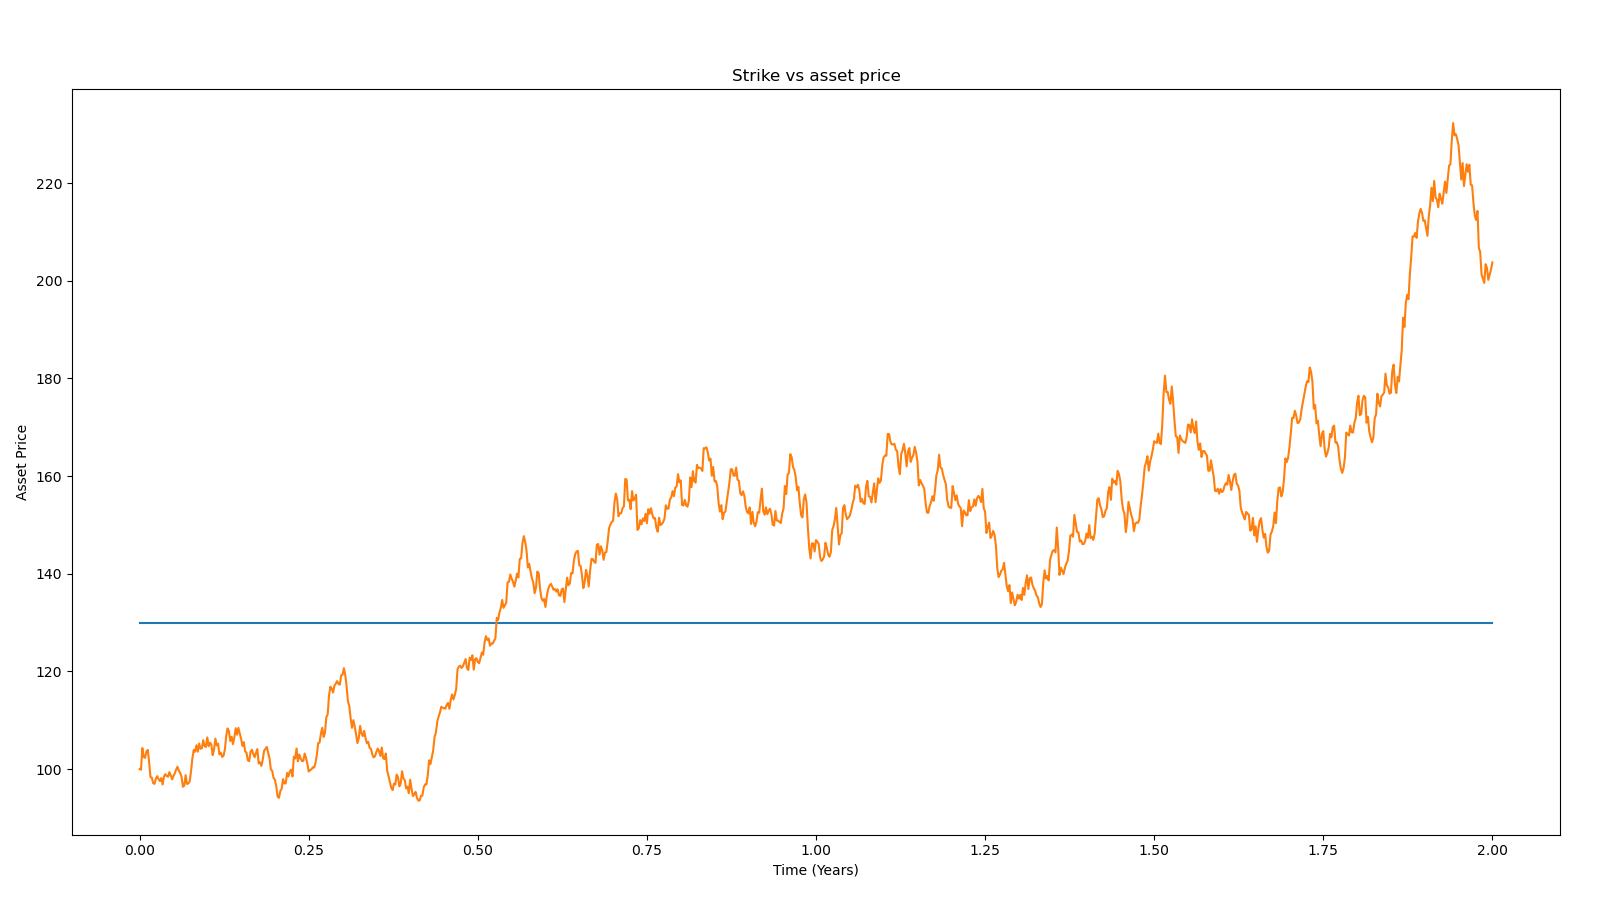
\includegraphics[width=12cm]{imgs/strike.png}
\end{frame}
\begin{frame}{Option Call}{Exemple où l'on ne fait pas valoir l'option}
  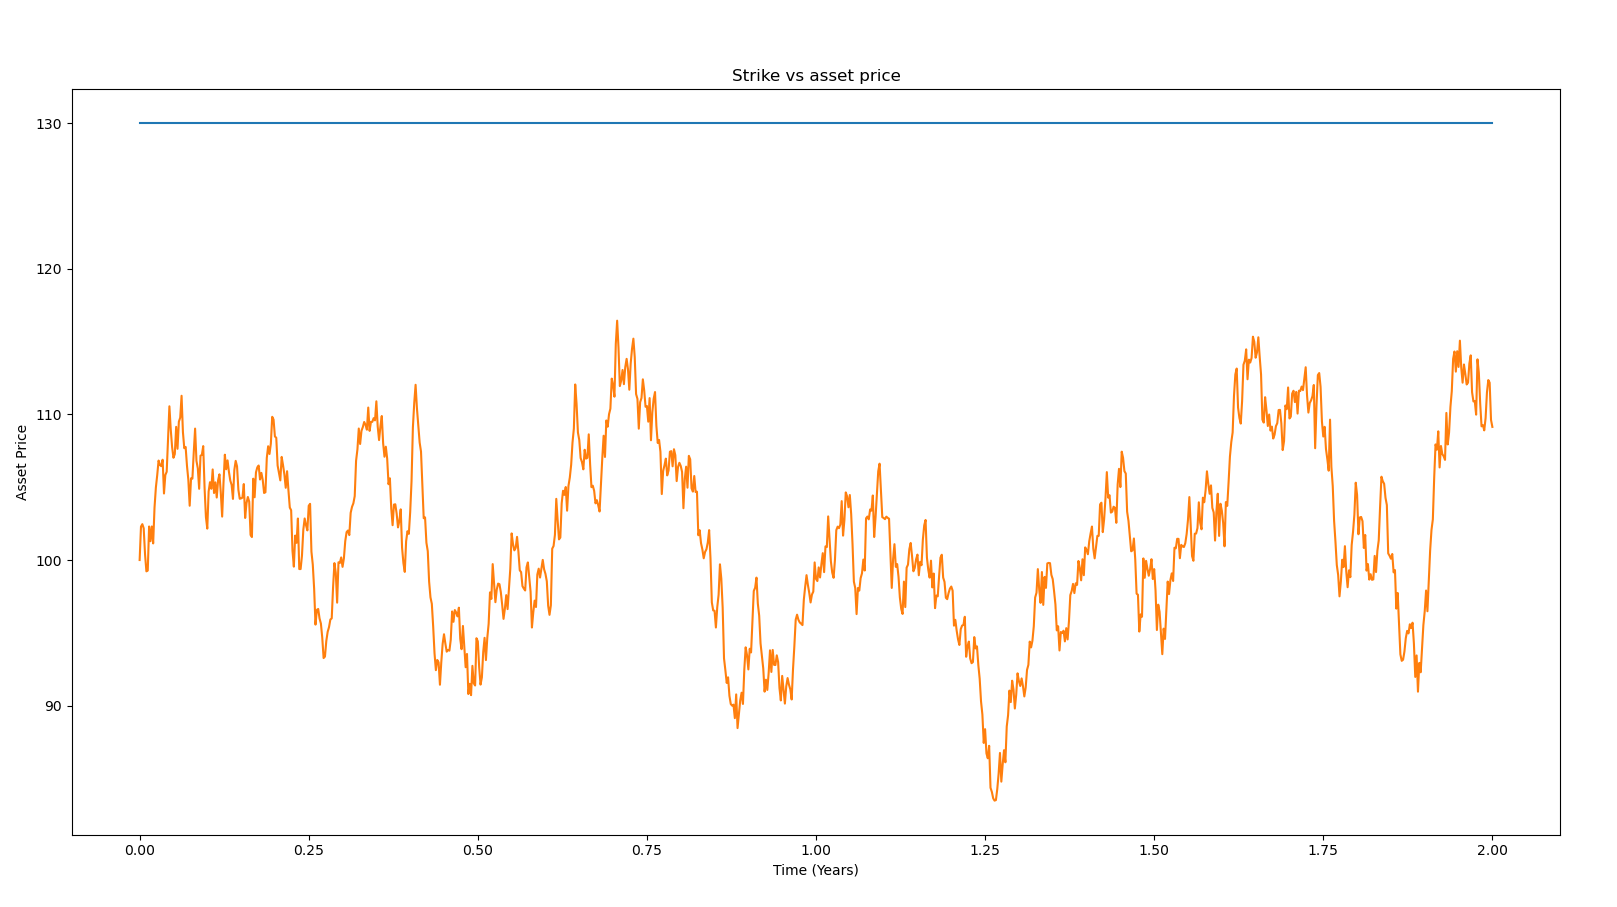
\includegraphics[width=12cm]{imgs/nostrike.png}
  \end{frame}
\begin{frame}{Processus Stochastique}
  \begin{block}{Définition}
    On appelle processus stochastique la donnée
    \begin{equation}
      X = (\varOmega, \mathcal{F}, \left(  X_{t} \right)_{t\in T}, \mathbb{P})
    \end{equation}
    où $ \varOmega $ est un ensemble, $ \mathcal{F} $ est une $\sigma$-algèbre sur $ \varOmega $, $\mathbb{P}$ est une mesure de probabilité sur $ \left( \varOmega , \mathcal{F} \right)$ et $T \subset \mathbb{R}^{+}$ (représente le temps).
    Enfin, $\left( X_{t} \right)_{t\in T} $  est une famille de variable aléatoire indexée par $ T $.
  \end{block}
\end{frame}
\begin{frame}{Mouvement Brownien}
  \begin{block}{Définition}
    Un processus $ B = (\varOmega, \mathcal{F}, \left(  X_{t} \right)_{t\in T}, \mathbb{P} ) $ à valeurs réelles est un mouvement brownien si
    \begin{subequations}
      \begin{equation} B_{0} = 0 \qquad \mathbb{P}-p.s \end{equation}
      \begin{equation} \forall s \in \left[0, t\right], \qquad B_{t} - B_{s} \indep \mathcal{F}_{s} \end{equation}
      \begin{equation} \forall s \in \left[0, t\right], \qquad B_{t} - B_{s} \sim \mathcal{N} \left( 0, t-s\right)\end{equation}
      \end{subequations}
    \end{block}
    Le mouvement brownien est donc un type particulier de {\em marche aléatoire}.
\end{frame}
% \begin{frame}{Explication et représentation du problème}
%   \includegraphics<2>[width=7.5cm]{imgs/overunder.png}
%   \hfill
%   \hfill \includegraphics<2>[width=7.5cm]{imgs/under.png}
% \end{frame}
\begin{frame}{Le modèle de Black-Scholes}
  \begin{block}{Définition}
    On va choisir de modéliser le marché en utilisant le processus stochastique satisfaisant l'équation stochastique suivante
    \begin{equation}
      \begin{cases}
        dX_{t} = \mu X_{t} dt + \sigma X_{t} dB_{s} \\
        X_{0} = 0
      \end{cases}
      \end{equation}
      est l'équation de Black-Scholes. \\
    \end{block}
    \pause
    \begin{alertblock}{}
    Le but va donc être de comprendre ce processus de manière plus globale, il nous faut donc une intégrale de la forme
    \[
      \int_0^{T} dX_{t} = \int_0^{T} \mu X_{t} dt + \int_{0}^{T} \sigma X_{T} dB_{t}
    \]
  \end{alertblock}
  \pause
  Le but va donc maintenant être de définir cette intégrale
\end{frame}
% \begin{frame}{Présentation du modèle de Black-Scholes}
%   \begin{block}{Le Modèle}
%     On va choisir de modéliser le marché en utilisant le processus stochastique satisfaisant l'équation stochastique suivante
%     \begin{equation}
%       \begin{cases}
%         dX_{t} = \mu dt + \sigma dB_{s} \\
%         X_{0} = 0
%       \end{cases}
%     \end{equation}
%     Où $ \mu \in \mathbb{R}$, $ \sigma \in \mathbb{R^{+}} $, $ B_{s} $ représente le mouvement Brownien
%   \end{block}
% \end{frame}
% %
%\begin{frame}{Explication et représentation du problème}
%   \includegraphics<2>[width=7.5cm]{imgs/overunder.png}
%   \hfill
%   \hfill \includegraphics<2>[width=7.5cm]{imgs/under.png}
% \end{frame}
% \begin{frame}{Revenir au problème de départ}
%   On se remémore de l'équation
%   \[
%       \begin{cases}
%         dX_{t} = \mu dt + \sigma dB_{s} \\
%         X_{0} = 0
%       \end{cases}
%     \]
%     dont on comprend maintenant les termes. \\
%     Le but va donc être de comprendre ce processus de manière plus globale, il nous faut donc une intégrale de la forme
%     \[
%       I(f)(\omega) = \int_{0}^{T}f(\omega, t)dBt
%     \]
%   \end{frame}
%   \begin{frame}{Représentation d'un $X_t$ résolvant cette équation avec $\mu=10, \sigma=1$}
%    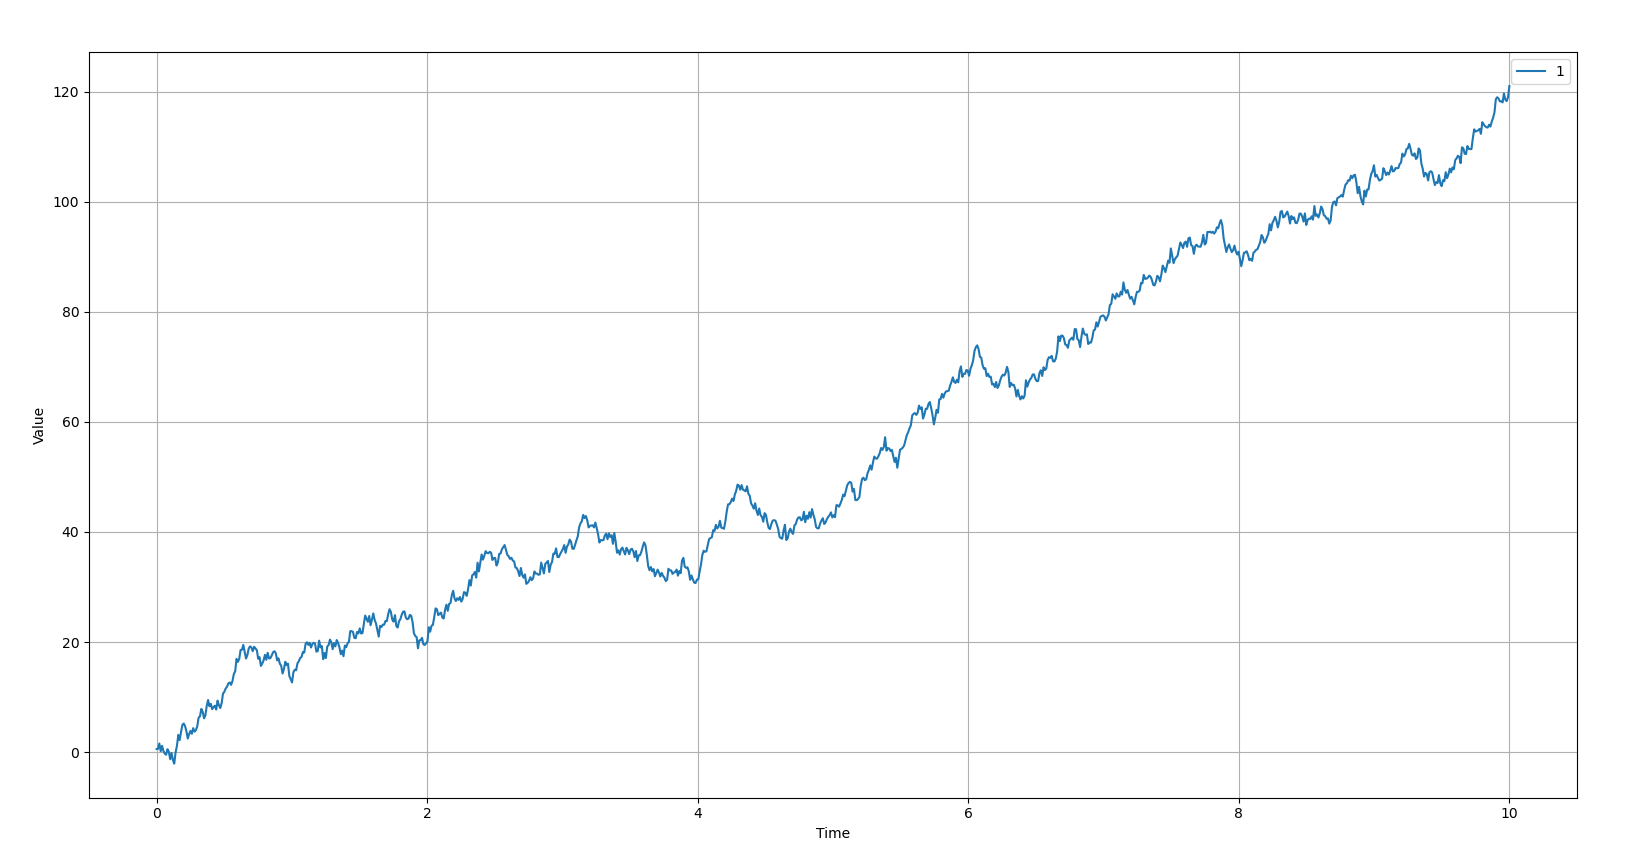
\includegraphics[width=10cm]{imgs/drift.png}
%  \end{frame}

 \begin{frame}{Représentation de cinq $X_{t}$ résolvant cette équation}
   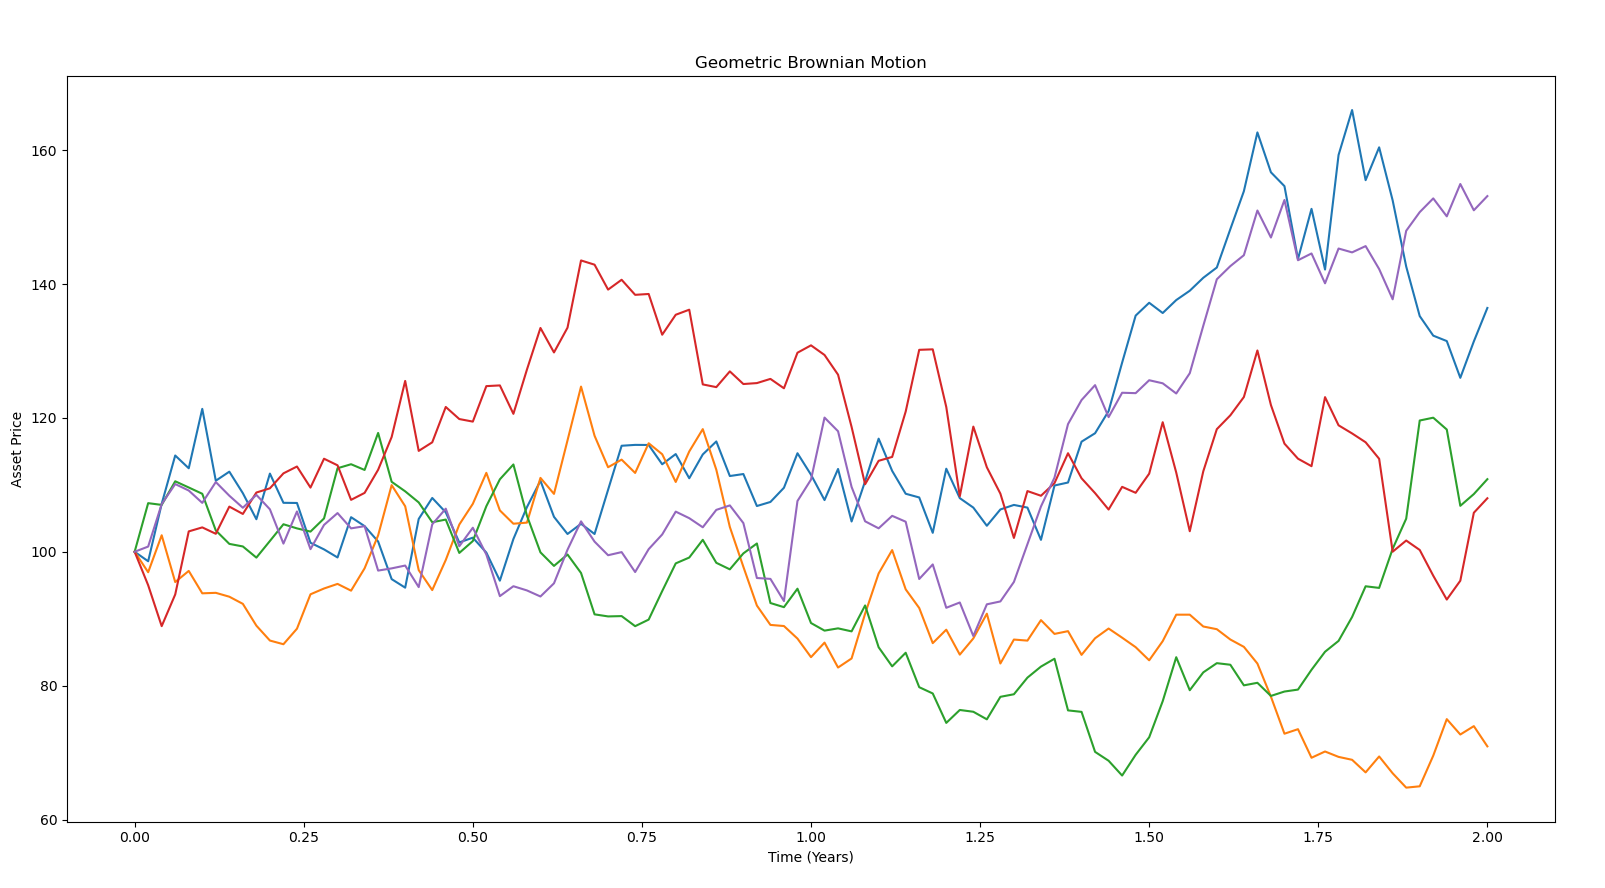
\includegraphics[width=12cm]{imgs/bs5.png}
 \end{frame}
 \begin{frame}{Construction de l'intégrale d'Itô}
   \begin{block}{Définition}<1->
     On définit $\mathcal{H}^{2}$ comme étant l'espace des fonctions mesurables et adaptées respectant la condition d'intégrabilité \\
     \[
       \mathbb{E}\left[\int_{0}^{T}f^{2}(\omega, t) dt \right] < \infty
     \]
   \end{block}
    \begin{block}{Propriété de base de l'intégrale}
     On aimerait que notre intégrale aient les propriétés suivantes, \\
\iffalse [ [ \fi     D'abord, si $ f(\omega, t) = \1_{\left] a; b \right]} $ on aimerait
     \[
       I(f)(\omega) = \int_{a}^{b}f(\omega, t) dB_{t} = B_{b} - B_{a}
     \]
   \end{block}

 \end{frame}
 
 \begin{frame}{Définition de l'intégrale d'Itô sur $\mathcal{H}^2_0$}
      \begin{block}{Définition}
     On définit maintenant $\mathcal{H}^{2}_{0}$ comme le sous-ensemble des fonctions dans $\mathcal{H}^{2}$ telles que celles-ci soient de la forme \iffalse [[ \fi
     \[
       f(\omega, t) = \sum_{i=0}^{n-1}a_{i}(\omega) \1_{\left] t_{i} ; t_{i+1} \right] }
     \]
     \end{block}
     \begin{block}{Définition}<2->
       Soit $ f \in \mathcal{H}^{2}_{0} $ on va définir l'intégrale d'Itô comme étant
       \[
         I(f)(\omega) = \sum_{i=0}^{n-1} a_{i}(\omega)\left( B_{t_{i+1}} - B_{t_{i}} \right)
       \]
     \end{block}
     \pause
   En fait, comme $ \mathcal{H}^{2}_{0}$ est dense dans $\mathcal{H}^{2}$, on peut définir l'intégrale sur tout $\mathcal{H}^2$
   \end{frame}
   \begin{frame}{Lemme d'Itô}{Cas simple}
     \begin{block}{Lemme d'Itô}
       Avec $f: \mathbb{R} \rightarrow \mathbb{R} $ est de classe $ \mathcal{C}^{2} $, alors
       \begin{equation}
         f(B_{t}) = f(0) + \int_{0}^{t}f'(B_{S})dB_{S} + \frac{1}{2}\int_{0}^{t} f''(B_{s})ds
       \end{equation}
     \end{block}
     \pause
     On note la similarité entre cette équation et le théorème fondamental de l'analyse, à ceci près qu'une intégrale de la dérivée seconde de f s'invite dans l'équation
     \pause
     \begin{block}{Lemme d'Itô, avec plusieurs variables}
       Soit $f\in \mathcal{C}^{1, 2}(\mathbb{R}^{+} \times \mathbb{R})$, on a
       \begin{equation}
           f(t, B_{t}) = f(0, 0) + \int_{0}^{t}\frac{\partial f}{\partial x}(s, B_{s}) dB_{s} + \int_{0}^{t}\frac{\partial f}{\partial t}(s, B_{s}) ds + \frac{1}{2} \int_{0}^{t}\frac{\partial ^{2} f}{\partial x^{2}}(s, B_{s})
         \end{equation}
         \end{block}
     \end{frame}
     \begin{frame}{Lemme d'Itô, notation Shorthand}
       \begin{block}{Lemme d'Itô (notation)}
         Soit $f\in \mathcal{C}^{1, 2}(\mathbb{R}^{+} \times \mathbb{R})$, et $ X_{t} = f(t, B_{t})$ un processus stochastique, on écrira
         \begin{equation}
           dX_{t} = \frac{\partial f}{\partial x}(t, B_{t}) dB_{t} + \frac{\partial f}{\partial t}(t, B_{t}) dt + \frac{1}{2} \frac{\partial^{2}f}{\partial x^{2}}(t, B_{t}) dt
         \end{equation}
       \end{block}
     \end{frame}
     \begin{frame}{Lemme d'Itô}{Box-Calculus}
       \begin{block}{Box-Calculus}
         \begin{center}
           \begin{tabular}{|c|c|c|}
             \hline
             $\cdot$ & $dt$ & $dB_t$ \\
             \hline
             $dt$ & 0 & 0 \\
             $dB_{t}$ & 0 & $dt$ \\
             \hline
           \end{tabular}
         \end{center}
         \end{block}
       \end{frame}
   \begin{frame}{Lemme d'Itô}{Application à Black-Scholes}
     On reprend notre équation stochastique de Black-Scholes
     \begin{equation}
       dX_{t} = \mu X_{t} dt + \sigma X_{t} dB_{s}
     \end{equation}
     \pause
     et on s'intéresse à $d \ln X_{t}$ en y appliquant la formule d'Itô
     \[
       d \ln X_{t} = \frac{1}{X_{t}} \left( \mu X_{t} dt + \sigma X_{t} dB_{t} \right) - \frac{1}{2X_{t}^{2}} \left( \mu X_{t} dt + \sigma X_{t} dB_{t} \right) \left( \mu X_{t}dt + \sigma X_{t} dB_{t}\right)
     \]
     \pause
     ensuite, en appliquant le Box-Calculus, on voit qu'il est possible de simplifier cette dernière expression
     \begin{equation}
       d \ln X_{t} =  \mu dt + \sigma dB_{t} - \frac{\sigma^{2}}{2} dt
     \end{equation}
   \end{frame}
   \begin{frame}{Lemme d'Itô}{Application à Black-Scholes (suite)}
     \[
       d \ln X_{t} = \left( \mu - \frac{\sigma^{2}}{2} \right) dt + \sigma dB_{t}
     \]
     \pause
     On intègre ensuite de chaque côté de l'équation avec l'intégrale d'Itô
     \[
       \int_{0}^{T} d \ln \left(  X_{t} \right) = \int_{0}^{T} \left(\mu - \frac{\sigma^{2}}{2} \right) dt + \int_{0}^{T} \sigma dB_{t}
     \]
     \pause
     \[
       \ln \left(\frac{X_{t}}{X_{0}} \right) = \left( \mu - \frac{\sigma^{2}}{2} \right) T + \sigma B_{T}
     \]
     \pause
     \begin{equation} \label{lognor}
       X_{t} = \exp \left(  \left( \mu - \frac{\sigma^{2}}{2} \right) T + \sigma B_{T} \right)
     \end{equation}
   \end{frame}
   \begin{frame}{Lemme d'Itô}{Déduction de la formule de Black-Scholes}
     \begin{block}{Définition}
       Soit $Z \sim \mathcal{N}\left(0, 1 \right)$, et soient $\mu \in \mathbb{R}$ et $\sigma \in \mathbb{R}^{+}$, alors la variable définie par $ X = e^{\mu + \sigma Z}$ suit une loi log-normale.
     \end{block}
     On reprend donc \label{lognor} pour voir que
   \end{frame}
\end{document}
